% Advanced Programming 2025 - Project Report Template
% HEC Lausanne / UNIL
\documentclass[11pt,a4paper]{article}

% Packages
\usepackage[utf8]{inputenc}
\usepackage[T1]{fontenc}
\usepackage[english]{babel}
\usepackage{amsmath,amssymb,amsthm}
\usepackage{graphicx}
\usepackage{xcolor}
\usepackage{listings}
\usepackage{hyperref}
\usepackage[margin=1in]{geometry}
\usepackage{fancyhdr}
\usepackage{float}
\usepackage{caption}
\usepackage{subcaption}
\usepackage{tabularx}
\usepackage{array}
\usepackage{booktabs}
\usepackage{biblatex}
\usepackage{listings}
\usepackage{xcolor}
\addbibresource{references.bib} % Create this file for your references

% Code listing settings
\definecolor{codegreen}{rgb}{0,0.6,0}
\definecolor{codegray}{rgb}{0.5,0.5,0.5}
\definecolor{codepurple}{rgb}{0.58,0,0.82}
\definecolor{backcolour}{rgb}{0.95,0.95,0.92}

\lstdefinestyle{pythonstyle}{
    backgroundcolor=\color{backcolour},   
    commentstyle=\color{codegreen},
    keywordstyle=\color{magenta},
    numberstyle=\tiny\color{codegray},
    stringstyle=\color{codepurple},
    basicstyle=\ttfamily\footnotesize,
    breakatwhitespace=false,         
    breaklines=true,                 
    captionpos=b,                    
    keepspaces=true,                 
    numbers=left,                    
    numbersep=5pt,                  
    showspaces=false,                
    showstringspaces=false,
    showtabs=false,                  
    tabsize=2,
    language=Python
}

\lstset{
  basicstyle=\ttfamily\footnotesize,
  columns=fullflexible,
  keepspaces=true,
  breaklines=true,
  frame=none,              % ← no box, no lines
  backgroundcolor=\color{gray!5},
  commentstyle=\color{green!50!black}
}
\lstset{style=pythonstyle}

% Header and footer
\pagestyle{fancy}
\fancyhf{}
\rhead{Advanced Programming 2025}
\lhead{Project Report}
\rfoot{Page \thepage}

% Title page information - MODIFY THESE
\title{%
    \Large \textbf{Advanced Programming 2025} \\
    \vspace{0.5cm}
    \LARGE \textbf{Fantasy Premier League Team Optimizer} \\
    \vspace{0.3cm}
    \large Final Project Report
}
\author{
    Mattia Comisetti \\
    \texttt{mattia.comisetti@unil.ch} \\
    Student ID: 20437588
}
\date{\today}

\begin{document}

\maketitle
\thispagestyle{empty}

\begin{abstract}
\noindent
Fantasy Premier League (FPL) is a popular online game in which participants select football players under strict budget and squad constraints, with success often attributed to a combination of analysis, intuition, and luck. This project examines whether data-driven machine learning models can systematically outperform average human strategies in FPL decision making. Using a unified, multi-season dataset spanning nine Premier league seasons (2016-17 to 2024-25), three machine learning models (Random Forest, XGBoost, and LightGBM) were trained to predict player points for the subsequent gameweek. These predictions were then integrated into a linear programming optimizer that constructed valid FPL squads, while respecting in-game constraints. 

Model performance was evaluated at both the point-prediction level using standard regression metrics, and in terms of real-world outcome by comparing the actual FPL points each model scored for a given gameweek to the global FPL manager average. The results indicate that LightGBM consistently outperformed the other models, achieving the lowest validation error, and generating teams that scored considerably better than the average FPL manager. Overall, this study demonstrates that a well-designed machine learning pipeline can meaningfully compete with the average FPL player and could be used to improve FPL decision making. 

\end{abstract}

\vspace{0.5cm}
\noindent\textbf{Keywords:} Data Science, Python, Machine Learning, Fantasy Premier League, RandomForest, XGBoost, LightGBM

\newpage
\tableofcontents
\newpage

% ================== MAIN CONTENT ==================

\section{Introduction}
\label{sec:introduction}

Fantasy Premier League (FPL) is a popular fantasy sports game based off of the English Premier League, which is played by over 11 million people ever year. Players assemble squads of professional footballers, while respecting a fixed budget and score points based off the real-world performance of these players in Premier League football games. FPL is a game riddled with different strategies. Some believe that success depends on watching the games and having an intuition or “feeling” whereas others believe in a more statistical approach, relying on the underlying data in order to make squad-building decisions. These discussions motivate a broader question central to sports analytics: to what extent can data-driven methods meaningfully improve decision making in environments characterized by uncertainty and high variance? 

In FPL, each manager selects a squad of 15 players within a 100 million budget at the start of the season. Out of these 15 players, 11 are selected to start every week, and will have the opportunity to score points for that Gameweek (GW). There are certain formation constraints regarding the team that can be put forward every week: there can only be one goalkeeper, and there must be a minimum of three defenders, two midfielders, and one forward. Player prices may vary throughout the season according to popularity and perceived performance potential, which is important as managers are allowed to make one transfer per gameweek. As a result, FPL represents a constrained optimization problem in which managers must balance expected performance, budget limitations, team composition rules, as well as future planning. 

The specific problem addressed in this project is to evaluate the extent to which statistical learning models can outperform average human decision making in FPL. To this end, a machine learning system is developed that learns patterns from past historical data spanning nine seasons (2016-17 to 2024-25), sourced from the publicly available Vaastav Fantasy Premier League dataset. These patterns are then applied to the ongoing 2025-26 season, in order to predict player performance on a gameweek-by-gameweek basis. Using these predictions, the machine learning models will construct optimized FPL teams in gameweek two, and will transfer exactly one player every gameweek thereafter, mirroring the constraints faced by real life FPL managers. 

In order to reduce model-specific bias and ensure a fair comparison, three tree based machine learning models are used: Random Forest, LightGBM, and XGBoost. Each model is trained to predict a player’s points in the following gameweek, and is evaluated based off of point-level predictive accuracy, as well as their real-world decision quality, measured by the actual FPL points scored by the optimized teams. The strategies developed are further compared against the global FPL average in order to determine whether data-driven approaches can deliver consistent performance gains over typical human strategies.\\

Accordingly, the project seeks to answer the following research question:\\

\textbf{Which prediction models perform best for predicting an optimal Fantasy Premier League team: Random Forest, LightGBM, or XGBoost?}\\

The remainder of this report is structured in the following way. Firstly, section 2 will review relevant literature on sports performance prediction and fantasy sport analytics. Then, section 3 will go over the methodology, including the data sources, the feature engineering process, as well as the modeling methodology. Section 4 will then present the empirical results, including predictive performance metrics and season-level performance. Section 5 discusses the implications, limitations, and interpretability of the findings, and, finally, section 6 will conclude the report and include the outline for potential directions for future research.   

\section{Literature Review / Related Work}
\label{sec:literature}

Sport analytics is a popular field, and the prediction of player and team performance is a subject that has been widely studied within the field. Approaches range from traditional statistical methods to more advanced machine learning techniques, and although early work relied on linear and logistic regression models, more recent studies have increasingly adopted machine learning algorithms, including Random Forests, gradient boosting methods, as well as, in some cases, neural networks, to capture non-linear relationships and interactions present in structured sports data.

The vast majority of these studies base themselves off of publicly available datasets, which play a central role in enabling empirical research. These datasets typically include match and player-level statistics obtained from official Premier League API’s, aggregated season summaries, as well as open-source repositories that compile performance metrics across multiple seasons. 

Although there is already a large amount of research in this area, much of the existing literature focuses on single model approaches and rely on limited feature sets or datasets spanning only one or two seasons. This restricts the model’s ability to assess how well these models generalize in a wide variety of competitive contexts and evolving league dynamics. This is particularly relevant for FPL, where team tactics, player roles, and scoring distributions change considerably over time, and where data availability and feature definitions change across seasons. 

A closely related recent study is the OpenFPL framework, which proposes an open-source approach to forecasting FPL points using ensemble regression models trained on publicly available FPL statistics. While this work does demonstrate strong point level predictive performance, its primary focus remains on player-level forecasting accuracy rather than on the decision-making process faced by FPL managers. On the other hand, the present project extends beyond point-level prediction by embedding machine learning outputs into a constrained optimization process that reflects the actual decision environment faced by FPL managers. The models are then tested on the same historical data and on the same future season, and their success is measured by the total points scored by the team they generate. This makes the evaluation more realistic as it reflects how managers think throughout a season and enables a more effective comparison of statistics versus human intuition. 

Building on these considerations, this project constructs a unified, multi-season dataset and conducts a systematic comparison of three tree-based machine learning models within a consistent experimental framework. By jointly evaluating Random Forest, LightGBM, and XGBoost models using identical data and conditions, as well as assessing both prediction quality and downstream performance, this study offers clearer empirical insights into which model is best suited for structured, low frequency sports prediction tasks such as FPL. 

\section{Methodology}
\label{sec:methodology}

\subsection{Data Description}
Initially, the objective was to retrieve historical FPL data directly from the official FPL API. However, the API only processes the current season, and does not offer historical records of the past ones. To overcome this limitation, historical data was retrieved from the Vaastav Fantasy Premier League repository. It is an open source dataset that provides player and gameweek level FPL statistics for all seasons since the 2016-17 season, up to gameweek 9 of the 2025-26 season at the time of the analysis. 

The resulting data set contains approximately 230’000 observations and around 55 variables, with slight differences in features depending on the season. Each row corresponds to a player’s performance in a specific gameweek, which produces a structured tabular data set at the player-gameweek level. Difficulties arose due to the heterogeneous nature of the data set. Several advanced performance metrics such as expected goals, bonus points, and further detailed statistics are only available in more recent seasons, particularly from the 2022-23 season onward. This is due not only to the repository, but also to rule changes and the integration of new features in the Fantasy Premier League game. In addition, the dataset is highly imbalanced between players, as regularly starting players accumulate long sequences of gameweek observations, whereas bench players often exhibit runs of zero-minute appearances. 

Although the observations do follow a temporal order within each season, the dataset does not constitute a regular time series. Players miss gameweeks due to injuries, rotation, suspension, or transfers, which leads to irregular temporal spacing. Furthermore, many numerical variables, such as minutes played, total points, goals scored, and ICT-based metrics show a strong right skewness, with a large mass at zero and occasional extreme outliers due to exceptional performances. The data set is particularly well suited to tree-based ML models due to these characteristics, as they are robust to sparsity, missing values, and nonlinear interactions and less reliant on evenly spaced temporal sequences. 

The Vaastav FPL dataset contains a wide range of player, and match level statistics that describe performance, context, and underlying contributions. Certain core variables include minutes played and total\_points, which serve as the basis for both availability modeling as well as target construction. Attacking and defensive statistics such as goals scored, assists, clean sheets, goals conceded, and saves are complemented by negative scoring events, including yellow and red cards, own goals, and penalties missed. As stated above, more recent season also include more advanced metrics such as expected goals (xG), expected assists (xA), expected goal involvements (xGI), and expected goals conceded (xGC), which provide deeper insight into chance quality and defensive strength. These are complemented with FPL specific statistics such as bonus points, BPS, ICT index, creativity, threat and influence. These statistics capture broader contributions beyond raw scoring events, which can be useful when trying to predict future points. Contextual information is also included, and include variables such as team and opponent identifiers, as well as home-away indicators. Economic and popularity signals are reflected in the player price, ownership rates, and transfer activity, and can give the model a small insight into more qualitative information. Finally, availability descriptors such as starting and player injury status help model playing time uncertainty. Together, these features provide a comprehensive statistical representation of each player’s performance, and context for every gameweek. 

Quite a few data quality challenges had to be addressed prior to modeling. As missing values are frequent, notably for players who did not feature in each gameweek, there are several zeros or missing entries across many performance variables. There is also the issue of structural missingness, as advanced metrics are unavailable for earlier seasons. Outliers are also common, driven by both exceptional performances and adverse events such as red cards. Furthermore, inconsistencies in variable naming, data formats, and identifier encodings across seasons required careful normalization. All of these features call for systematic cleaning, schema harmonization, and feature engineering to ensure consistency and suitability for machine learning analysis. 


\subsection{Approach}
This project employs three tree-based machine learning models: Random Forest, XGBoost, and LightGBM. These models were selected due to their strong empirical performance on structured, tabular datasets, as well as their ability to capture complex nonlinear relationships without requiring dense or regularly spaced time-series inputs. When comparing to deep learning approaches, tree-based methods are more robust in settings characterized by sparse observations, relatively low temporal resolution, and heterogeneous feature availability, which are all defining properties of FPL data. 

The modeling framework follows a supervised learning setup in which each observation corresponds to a (player, season, gameweek) tuple enriched with engineering features. The target variable is defined as the player’s total FPL points in the following gameweek, requiring a forward-looking prediction consistent with real-world decision making. Feature engineering includes rolling historical aggregates at the player and team level, contextual indicators such as home advantage and opponent strength estimates, and cumulative season statistics, computed purely from past information to avoid data leakage. 

The evaluation of the models relied on standard regression metrics, notably Mean Absolute Error (MAE) and Room Mean Squared Error, which quantify point-level predictive accuracy, as well as the coefficient of determination ($R^2$), which measures the proportion of the variance in the next-gameweek points explained by the model. A temporarily held out validation window, which consists of gameweeks 1-9 of the 2025-26 season is used to ensure a realistic, forward-looking assessment. The evaluation design avoids data leakage, mirrors the information constraints faced by FPL managers, and allows for a fair comparison of model generalization performance. 


\subsection{Implementation}
The entire pipeline is implemented in Python, using a modular architecture built with widely used scientific and machine learning libraries. Data manipulation and preprocessing are handled with Pandas and Numpy. Model training and evaluation rely on scikit-learn for the Random Forest baseline, and on the LightGBM and XGBoost libraries for the gradient-boosted tree models. Squad optimization is formulated as a linear programming problem and solved using the PuLP optimization framework. Further utilities include requests for API access, joblib for model persistence, and matplotlib for result visualization.

The pipeline is organized into a sequence of scripts, each representing a distinct stage in the workflow. Historical data is ingested and handled by a dedicated script that builds unified player and gameweek level tables across all the seasons. Feature engineering is performed in a separate model that constructs ML ready player-gameweek feature matrices. The models are then trained and compared in a standalone training script that fits all models, generates predictions for each player, and evaluates their separate predictive performance. These predictions are then consumed by an optimization module that constructs FPL squads across multiple gameweeks, while respecting all the constraints. Finally, an evaluation module retrieves actual FPL outcomes via the official FPL API and compares the realized performance of each model’s strategy against the global FPL average. A final script then creates figures and tables of the results.

The implementation is organized into modular components that cover data preparation, feature engineering, model training, optimization, and evaluation. Player and match data are initially standardized across seasons, after which rolling player and team features are constructed and used to train predictive models. The resulting predictions are integrated into an optimization process that respects FPL constraints. This structure allows the entire pipeline to remain transparent, reproducible, and easy to extend.


\section{Results}
\label{sec:results}

\subsection{Experimental Setup}
The entire project was carried out in the cloud based Visual Studio Code environment using standard multi-core CPU resources, without GPU acceleration. This setup was well suited to the tree-based models used in this study, which do not rely on specialized hardware. The project was conducted entirely in Python 3.11, with hyperparameters selected with the goal of balancing predictive performance and computational efficiency. The Random Forest model was trained using 400 trees with a minimum leaf size of 5 observations, while both XGBoost and LightGBM used 500 boosting iterations with a learning rate of 0.05, with LightGBM limited to 31 leaves and XGBoost to a maximum tree depth of eight. Hyperparameters were chosen to reflect standard, well-performing configurations for each model family rather than enforcing identical parameter counts. This is because tree counts and boosting iterations are not directly comparable across Random Forest and gradient boosting methods.The rest of the configuration remained the same across models to allow fair comparison.   

\subsection{Performance Evaluation}
\subsubsection{Predictive performance on the validation set}
This section evaluates the performance of the three proposed ML models in forecasting FPL points for the next gameweek. As discussed above in the methodology, each model was trained on the historical player-gameweek data extracted from the seasons 2016-17 until 2024-25, and then evaluated on a temporarily held out validation set made up of the first nine gameweeks in the 2025-26 season. All data splits were performed in a chronological order, to avoid data leakage and to ensure the model reflects a realistic forecasting scenario faced by FPL managers. 

Model performance is assessed using three complementary regression-based metrics, each offering a distinct perspective on predictive accuracy. Mean Absolute Error (MAE) captures the average magnitude of prediction errors, while average Root Mean Squared Error (RMSE) places greater emphasis on large deviations, thereby penalizing extreme mispredictions more strongly. The coefficient of determination ($R^2$) measures the proportion of variance in next gameweek points explained by the model. Together, these metrics provide a robust assessment of point-level forecasting performance. In addition, to ranking and decision-oriented evaluations are considered later in the analysis, as the accurate identification of high performing players is ultimately more relevant for FPL decision making than exact point prediction alone.

\begin{table}[H]
\centering
\caption{Point level predictive performance on the validation set}
\label{tab:performance}
\begin{tabular}{|l|c|c|c|c|}
\hline
\textbf{Model} & \textbf{Valid\_MAE} & \textbf{Valid\_RMSE} & \textbf{Valid\_$R^2$} & \textbf{Spearman\_Rho}\\
\hline
RandomForest & 1.360 & 2.076 & 0.254 & 0.725 \\
XGBoost & 1.169 & 2.080 & 0.251 & 0.719\\
LightGBM & 1.130 & 2.033 & 0.284 & 0.729\\
\hline
\end{tabular}
\end{table}
Clear differences in predictive performance emerge across the three models. LightGBM consistently outperforms both RandomForest and XGBoost on all reported metrics,  achieving the lowest MAE and RMSE as well as the highest $R^2$ value. A validation MAE of 1.130 indicates that, on average, the LightGBM model’s predictions deviate from the actual next gameweek FPL points by slightly more than one point per player, which is notable given the inherent randomness and volatility of football outcomes. XGBoost exhibits statistics that are marginally worse than LightGBM, with a higher MAE of 1.169 and a slightly lower $R^2$ than Random Forest. While LightGMB achieves superior point-level predictive accuracy, all three models exhibit comparable ranking performance, as reflected by similar Spearman correlation coefficient (ranging from 0,719 to 0,729). This suggests that improvements in absolute prediction accuracy do not necessarily translate into substantially better player ranking, which may have implications for downstream FPL-decision making. However, strong performance alone is not sufficient to assess model reliability. It is also essential to examin whether these performance differences arise from genuine generalization or from overfitting to the training data. 

To further assess this overfitting, the difference between training and validation MAE was examined for each model. Overfitting is a phenomenon that occurs when a model captures an excessive amount of noise or idiosyncratic patterns in the training data, that do not generalize to unseen observations. The larger the discrepancies between the training and the validation error, the higher the risk of overfitting behavior. The figure below visualizes this comparison between models. 

\begin{figure}[H]
    \centering
    \includegraphics[width=0.5\linewidth]{Train_vs_Valid_MAE.png}
    \caption{Train vs Valid MAE (Overfitting check)}
    \label{fig:train_valid_mae}
\end{figure}

LightGBM exhibits the lowest gap between training and validation MAE, indicating strong generalization and limited overfitting. XGBoost shows a moderate discrepancy, suggesting some degree of overfitting. In contrast, Random Forest displays a large gap, with very low trainibg error but substantially higher validation error, consistent with pronouced overfitting and weaker generalization performance.

Overall, these results identify LightGBM as the most reliable model for point-level FPL prediction under a realistic temporal validation setup. The gradient boosting framework it uses appears particularly effective at capturing non-linear relationships and feature interactions in structured, sparse FPL data, while maintaining a strong generalization performance. 

\subsubsection{Decision Performance at the Season Level}
As important as point-level prediction accuracy may be, the ultimate objective of this project is to assess to what extent improved predictions translate into improved FPL decision making. To evaluate this, each model’s predictions were used in an optimization framework that generates weekly FPL teams under realistic game constraints, including budget limits, squad composition rules, and restricted transfers. This resulted in each model generating a 15-man squad at the start of the year (in gameweek two) and selecting 11 players every week to score points, while being allowed to transfer in and out one player per week. The generated teams were evaluated using the actual FPL points the team would have scored in that gameweek, obtained from the official FPL API.

Table~\ref{tab:season_performance} reports the total and average points scored by each model’s optimized team between the gameweeks 2 and 12 of the 2025-26 season, which are then compared to the global FPL average over the same period. The evaluation covers gameweeks 2 to 12 as predictions can only be generated from gameweek 2 onwards, and extending further would risk forecasting too far ahead without incorporating newly observed information. 

\begin{table}[H]
\centering
\caption{Season-level performance of optimized teams compared to the FPL average (GW2--GW12, 2025--26)}
\label{tab:season_performance}

\begin{tabularx}{\textwidth}{l c >{\centering\arraybackslash}X c c}
\toprule
\midrule
\bottomrule
\textbf{Model} &
\textbf{Total Points} &
\textbf{Avg Points per Gameweek} &
\textbf{Delta vs FPL Avg} &
\textbf{Num Gameweeks} \\
\hline
RandomForest & 586.000 & 53.273 & 32.000 & 11 \\
XGBoost      & 572.000 & 52.000 & 18.000 & 11 \\
LightGBM     & 637.000 & 57.909 &  83.000 & 11 \\
FPL Average & 554.000 & 50.364 &   0.000 & 11 \\
\hline
\end{tabularx}
\end{table}
The results remain in line with the validation results, as the LightGBM model substantially outperforms the two other models as well as the global FPL average. Over the 11 gameweek evaluation window, the team generated by the LightGBM model scored 637 points, 83 more than the average FPL manager. The Random Forest and XGBoost teams also outperform the FPL average, albeit by a smaller margin. These results highlight the fact that modest improvements in predictive accuracy can drastically improve downstream decision quality.

These differences are further illustrated in Figure~\ref{fig:cumulative_points}, which plots cumulative team points over time per model.
\begin{figure}[H]
    \centering
    \includegraphics[width=0.5\linewidth]{Points_Over_time.png}
    \caption{Model Cumulative Points Over Time}
    \label{fig:cumulative_points}
\end{figure}

One can observe a consistent and widening performance gap between the LightGBM model and the other approaches. Rather than benefiting from a few isolated high scoring weeks, it seems that the LightGBM strategy is consistently able to outperform the other models, suggesting that its superior performance is driven by a sustained superior decision quality rather than short-term variance or luck. 

Figure~\ref{fig:weekly_points} provides a more granular view by comparing the points scored by each model week by week. 
\begin{figure}[H]
    \centering
    \includegraphics[width=0.5\linewidth]{Points_Per_Week.png}
    \caption{Points per Gameweek per Model}
    \label{fig:weekly_points}
\end{figure}
While all the models exhibit substantial week-to-week variability, unavoidable due to the inherent uncertainty of football outcomes, the LightGBM model appears to achieve higher peaks during strong gameweeks (notably around GW 6-7) while generally avoiding the lowest outcomes observed for the alternative models. In contrast, the Random Forest and XGBoost were unable to capitalize on strong gameweeks as well, and achieved values lower than the FPL average more often. Overall, the LightGBM model seems to deliver a more favorable balance between upside capture and downside control over the evaluation window. This relative consistency is a  valuable asset in FPL, where sustained performance across gameweeks is more impactful for long term success than isolated high scoring weeks. It must be noted that the particularly strong performance observed in gameweeks 6 and 7 may partially inflate the overall LightGBM score, suggesting that an evaluation over a longer time horizon would be necessary to assess the robustness of these results. 

\section{Discussion}
\label{sec:discussion}

\subsection{What Worked Well}
One of the most important findings of this project is that the three models outperformed the average FPL manager over the evaluated gameweeks. This result is particularly impressive as the models operated under stricter constraints that a human FPL manager. For instance, they did not use special FPL chips, such as Triple Captain, Free hit, or Bench Boost, nor were they able to directly incorporate qualitative data such as injury reports, tactical speculation, or information gained from press conferences. Although some of these qualitative aspects could be somewhat integrated into the model through the previous weeks “transfer in” and “transfer out” statistics, which specified if FPL managers transferred a player in or out of their squad, the model relied almost exclusively on structured historical data. Despite these limitations, the LightGBM, XGBoost and Random Forest models achieved a significantly higher score than the average FPL player, which shows that a purely data driven approach can produce a competitive decision-making performance.

There were several methodological choices that contributed to this success. First, training the models on a large, unified dataset spanning nine seasons allowed them to learn stable performance patterns across a wide range of player roles, team dynamics and competitive contexts. Secondly, using rolling and lagged features ensured that each prediction was based purely on the information available prior to that gameweek prevented data leakage and improved temporal generalization. The rolling feature also reduced the models bias toward the single previous game performance, which would have led it to selecting the best player over the past gameweek every time. Finally, embedding the ML predictions into a linear programming framework proved effective in translating point level forecasts into realistic squad selection decisions. This optimization step enforced the rules of the FPL game onto the ML models, which enabled the evaluation to reflect the actual decision environment faced by FPL players, rather than focusing only on an isolated prediction accuracy. 

\subsection{Challenges Encountered}
A major challenge throughout this project was the heterogeneity and incompleteness of the historical FPL dataset. The available features evolved considerably over time, with important variables such as expected goals (xG) and expected assists (xA) only being available from the 2022-23 season onward. This resulted in structural missingness, that unfortunately could not be resolved through simple imputation without introducing bias or artificial signal. To mitigate this issue, the feature engineering process prioritized robust variables that were consistently available across all seasons, while selectively incorporating more advanced features such as xG and xA only when they were present. Rather than backfilling or imputing these statistics for earlier seasons, the pipeline allowed the models to exploit the richer feature sets available in the more recent data, leveraging the ability of tree-based algorithms to handle missing values and heterogeneous feature availability naturally. A further issue related to the inherent structure of the database was ensuring consistent player and team identifiers across seasons. This required careful normalization and cross referencing, especially in more recent seasons where schema inconsistencies and naming changes were more frequent. 

A second major challenge came from the temporal structure of the data. Player participation in the Premier League is inherently irregular. Injuries, substitutions, suspensions, or transfers are all reasons a player may miss a gameweek, resulting in discontinuous observation sequences. This irregularity makes the data more difficult to handle for traditional sequence based or time-series models that assume evenly spaced observations. To address this issue, the modeling framework treated each player-gameweek observation as an independent supervised learning instance, enriched with rolling and lagged features, rather than relying on sequential architecture.

From a data engineering perspective, managing an end-to-end pipeline which covered data ingestion, feature engineering, model training, optimization, and evaluation also posed significant challenges. Without careful design, any errors introduced at the early stages could easily be propagated into later components. This risk was mitigated through a modular codebase that clearly separated responsibilities into different sections, and a single executable entry point (main.py), which ensured reproducibility, simplified debugging, and allowed individual components to be tested and refined independently.


\subsection{Comparison VS Initial Expectations}
The initial expectation of this project was that the gradient boosting models (LightGBM and XGBoost) would outperform the Random Forest model in predicting the next gameweek points per player, and hence, generate higher scoring teams. The results partly support this hypothesis. LightGBM consistently outperforms Random Forest across both predictive and downstream decision making metrics, achieving the lowest validation error, strongest generalization performance, and the highest cumulative team score compared to the FPL average. However, XGBoost shows mixed performance relative to Random Forest, improving point-level accuracy as measured by MAE, but failing to deliver consistent gains across other metrics such as RMSE, $R^2$, and most importantly, overall points scored. This may be due to XGBoost’s sequential boosting framework, which can amplify early model errors, particularly in noisy and non-stationary environments such as FPL data.

The magnitude of the performance gap is also noteworthy. XGBoost exhibited reasonable training performance, yet failed to generalize effectively during the early-season validation window, as reflected by the lower scoring season outcomes. This divergence suggests that not all tree-based models adapt equally well to rapidly shifting contexts, and highlights the fact that LightGBM appears better suited to capturing these dynamics, which resulted in more robust generalization and superior decision making quality. 


\subsection{Limitations}
Despite its strengths, the proposed approach had several important limitations. Firstly, the predictive framework only forecasts player points for the following gameweek and does not explicitly plan over longer horizons by accounting for fixture difficulty across multiple upcoming weeks. Furthermore, the optimization component does not model chip usage (triple captain or free hit) effectively, which limits its capabilities to imitate optimal FPL strategies over a full season. 

The model also relies exclusively on historical numerical data, and therefore ignores  qualitative information such as injury news or suspensions, factors which often play a crucial role in real-world outcomes. The evaluation window is relatively short, (GW1-GW9) meaning that results may be influenced by early-season volatility and may not yet fully reflect long term performance trends. 

Finally, even though LightGBM achieved the strongest results in the study, they are difficulty generalizable. Its performance depends on a specific feature set, hyperparameter choices, and validation period. As such, these findings should not be interpreted as universally optimal across all sports, seasons or league contexts.

\subsection{Surprising Findings}
One of the more unexpected findings was the weak generalization performance of XGBoost. Despite its reputation for tabular prediction tasks, it did not manage to translate its solid prediction level statistics into strong team scores, highlighting that model effectiveness does not only depend on algorithmic strength, but also its alignment with the data structure and feature engineering. Moreover, small differences in point-level prediction accuracy led to substantial differences in season level performance, underscoring the importance of evaluating models in terms of real-world decision outcomes rather than predictive measures alone. 

\section{Conclusion and Future Work}
\label{sec:conclusion}

\subsection{Summary}
This project aimed to investigate the extent to which statistical modeling and machine learning can be effective when it comes to decision making in FPL, a game often perceived as a balance between analysis, intuition, and chance. By assembling a large, multi-season dataset, this study developed a fully reproducible end-to-end pipeline for player-level point prediction, squad optimization, and real world performance evaluation.

Three tree-based ML models (Random Forest, XGBoost, and LightGBM) were trained to predict next gameweek FPL points using rolling player and team level features. These predictions were integrated into a linear programming optimizer that constructed valid FPL squads under realistic in game constraints. Model performance was then evaluated both through standard regression metrics on a temporarily held out validation window and through the actual FPL points scored by the optimized teams, benchmarked against the global FPL average score. 

The results clearly indicate that LightGBM outperformed both Random Forest and XGBoost in this setting. LightGBM achieved the lowest validation error, and generated teams that consistently outperformed the two other models, as well as the global FPL average. In contrast, the weaker generalization performance of Random Forest and XGBoost translated directly into inferior team scores, highlighting the importance of robust predictive accuracy when models are imbedded in downstream decision-making systems. Overall, these findings demonstrate that certain statistical models can significantly outperform average human-making decision in FPL, even without access to qualitative information or in-game advantages such as chips. 


\subsection{Future Directions}
While the results are encouraging, several extensions could improve both predictive accuracy and practical relevance. One improvement could be to explicitly model all the special FPL mechanics such as Free hit, Bench Boost, etc., which were intentionally excluded in this model to avoid inflating early-season performance. Incorporating these elements in a full-season simulation would allow the framework to reflect real FPL gameplay more closely. Furthermore, enriching the feature set with qualitative data such as injury reports could further enhance predictive accuracy. 

Methodically, future work could also focus on probabilistic forecasting instead of point estimates. Using Bayesian or quantile-based models would allow the optimizer to account for uncertainty and downside risk, enabling it to distinguish between high variance players and more consistent, reliable ones. Another promising direction is long term planning, where squad decisions are optimized based on expected performance over multiple upcoming gameweeks. 

Finally, from a scalability perspective, the pipeline could be extended to support rolling retraining throughout the season, which would allow models to adapt dynamically as the season went on. Although this study focuses on FPL, the pipeline is broadly applicable and could be adapted to other fantasy sports, betting contexts, or constrained decision making problems where predictions must be combined with real world constraints and evaluated over time. 


% ================== REFERENCES ==================
\newpage
\section*{References}
\addcontentsline{toc}{section}{References}

% If using biblatex (recommended)
% \printbibliography[heading=none]

% Or manually:
\begin{enumerate}
    \item Fantasy Premier League. (2025). Fantasy Football Gameweek History for entry 642722. Premier League Website, Retrieved from https://fantasy.premierleague.com/entry/642722/history
    \item FPL API. (2025). FPL Historical Dataset. Available at https://github.com/vaastav/Fantasy-Premier-League
    \item Fantasy Premier League. (2025). Fantasy Premier League player, team, and gameweek metadata (bootstrap-static). Available at: https://fantasy.premierleague.com/api/bootstrap-static/
\end{enumerate}

% ================== APPENDICES ==================
\newpage
\appendix
\section{Additional Figures}
\label{app:figures}

\begin{figure}[H]
    \centering
    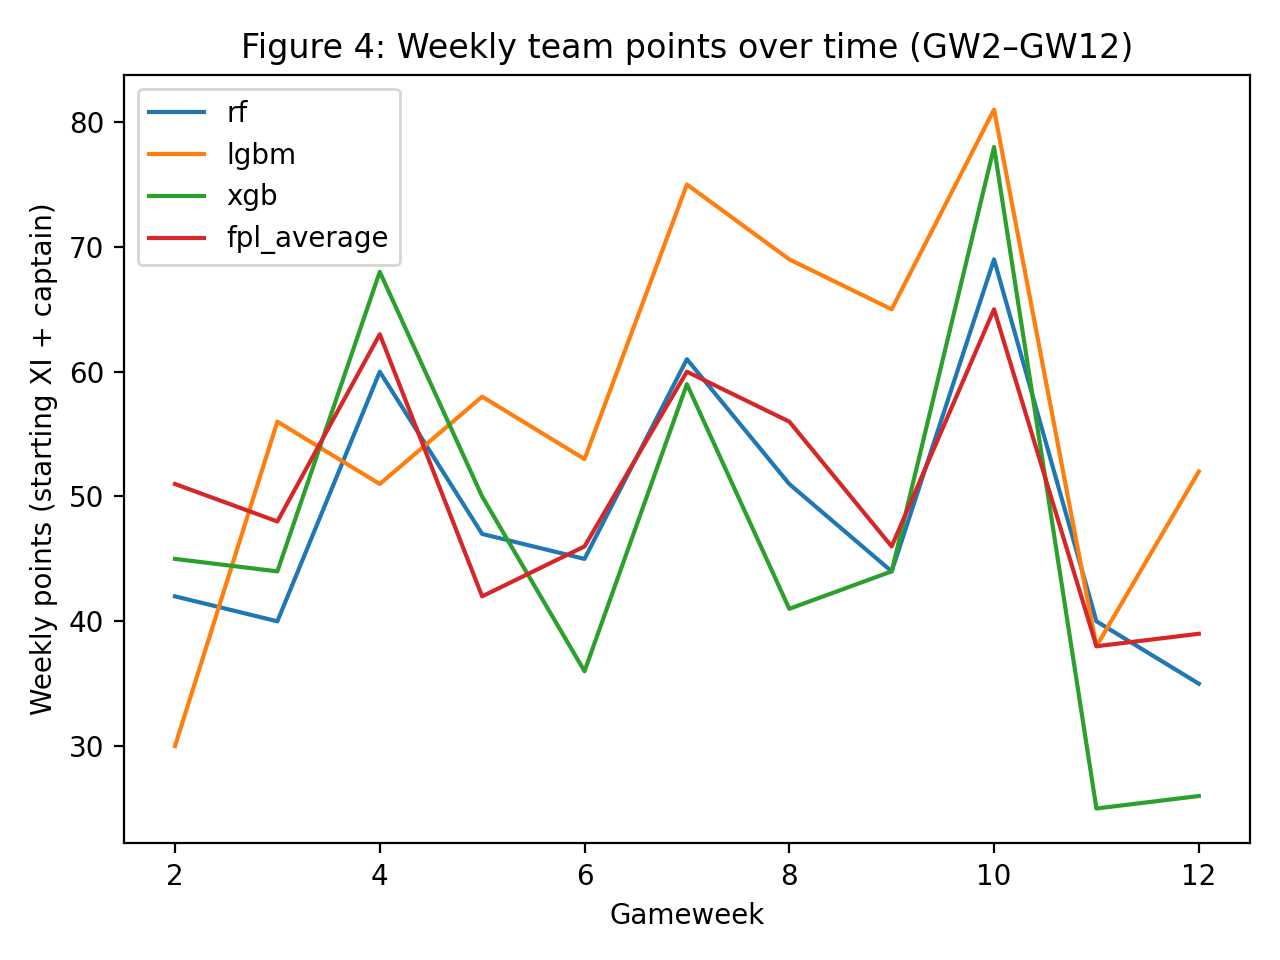
\includegraphics[width=0.5\linewidth]{image.png}
    \caption{Figure 4: Validation error per model}
    \label{fig:placeholder}
\end{figure}

\begin{table}[H]
\centering
\caption{Generalization Gap}
\label{generalization_gap}

\begin{tabularx}{\textwidth}{l c c c c c c}
\toprule
\textbf{Model} &
\textbf{Train\_MAE} &
\textbf{Valid\_MAE} &
\textbf{MAE\_GAP} &
\textbf{Train\_R$^2$} &
\textbf{Valid\_R$^2$} \\
\midrule
RandomForest & 0.698 & 1.356 & -0.658 & 0.699 & -0.033 \\
XGBoost      & 0.861 & 1.420 & -0.559 & 0.579 & -0.075 \\
LightGBM     & 1.028 & 1.138 & -0.110 & 0.398 &  0.228 \\
\bottomrule
\end{tabularx}
\end{table}

\section{Code Repository}
\label{app:code}


\noindent
\textbf{GitHub Repository:} \url{https://github.com/comisettim-eng/FPL-Team-Optimizer}
\subsection{Repository structure}

\begin{lstlisting}
FPL-Team-Optimizer/
  README.md
  requirements.txt
  environment.yml
  setup.py
  main.py
  project_report.md
  project_report.tex
  PROPOSAL.md

  data/
    raw/        # Raw FPL data fetched at runtime
    processed/  # Cleaned + feature-engineered datasets

  src/
    data/       # Data ingestion + feature construction
      __init__.py
      fetch_fpl_seasons_gw.py
      build_training_table_seasons.py

    models/     # ML training + comparison
      __init__.py
      train_compare_models.py

    optimize/   # Linear programming squad optimization
      __init__.py
      LP_team_optimizer_11P.py
      ML_season_optimizer_transfers_multi.py

    evaluate/   # Evaluation + reporting
      __init__.py
      compare_models_season_scores.py
      make_report_artifacts.py

  models/
    ml_models/  # Trained ML models (created at runtime)

  results/     # Generated outputs (tables, figures, predictions)
  Legacy/      # Deprecated / unused code (not executed)
  tests/
\end{lstlisting}

\subsection{Installation instructions}
This project is fully reproducible from a clean environment. All datasets, model artifacts, and evaluation results are generated automatically at runtime and are therefore not included in the repository.

To reproduce the full pipeline, the following steps are sufficient:
\begin{enumerate}
    \item Clone the repository.
    \item Create the Python environment using the provided \texttt{environment.yml} file.
    \item Run the main entry point \texttt{main.py}.
\end{enumerate}

The execution of \texttt{main.py} sequentially performs data collection from the Fantasy Premier League API, feature engineering, model training and comparison, season-long squad optimization using linear programming, and final evaluation against real FPL scores. All outputs (processed data, trained models, tables, and figures) are generated deterministically and saved to the appropriate runtime directories.

No manual intervention is required beyond running the main script.



\noindent

\begin{itemize}
    \item Repository structure
    \item Installation instructions
    \item How to reproduce results
\end{itemize}

\section{AI Tools Used}
ChatGPT was used to help correct and optimize code in this project, in order to make it more efficient in certain areas. It was also used to help reformulate, and translate parts of the report from french to english.

\end{document}